\documentclass[conference]{IEEEtran}
\pdfoutput=1    % For arXiv issues


% -------------------------- COLORBLIND COLORS -------------------------------
% Use color palettes for colorblind people from
% https://davidmathlogic.com/colorblind/#%23D81B60-%231E88E5-%23FFC107-%23004D40 or https://colorbrewer2.org/
\usepackage{xcolor}
\definecolor{wong-black}        {HTML}{000000}
\definecolor{wong-lightorange}  {HTML}{E69F00}
\definecolor{wong-lightblue}    {HTML}{56B4E9}
\definecolor{wong-green}        {HTML}{009E73}
\definecolor{wong-yellow}       {HTML}{F0E442}
\definecolor{wong-darkblue}     {HTML}{0072B2}
\definecolor{wong-darkorange}   {HTML}{D55E00}
\definecolor{wong-pink}         {HTML}{CC79A7}

% -------------------------- PACKAGES -------------------------------

\usepackage{url}
\def\UrlBreaks{\do\/\do-}   % Line breaks of long URLs in biblatex bibliography (https://tex.stackexchange.com/questions/134191/line-breaks-of-long-urls-in-biblatex-bibliography)

\usepackage{hyperref} % Working hyperlink (https://www.overleaf.com/learn/latex/Hyperlinks)
\hypersetup{
    colorlinks=true,
    citecolor=wong-green,
    linkcolor=wong-darkblue,
    filecolor=wong-pink,      
    urlcolor=wong-black,
    pdfpagemode=FullScreen,
    }

% Use these to always use Fig. and Sec. instead of worrying about Figure, Fig, Fig. etc in the document
\newcommand{\figref}[1]{Fig.~\ref{#1}}
\newcommand{\secref}[1]{Sec.~\ref{#1}}

\usepackage{cite}
\usepackage{amsmath,amssymb,amsfonts}
\usepackage{algorithmic}
\usepackage{graphicx}
\usepackage{textcomp}
\usepackage[nolist, nohyperlinks, printonlyused]{acronym} % For consistent acronyms

\def\BibTeX{{\rm B\kern-.05em{\sc i\kern-.025em b}\kern-.08em
    T\kern-.1667em\lower.7ex\hbox{E}\kern-.125emX}}
    
\newcommand\nnfootnote[1]{  % Footnote without hyperref association (https://tex.stackexchange.com/questions/415625/avoiding-hyperref-warning-ignoring-empty-anchor)
  \begin{NoHyper}
  \renewcommand\thefootnote{}\footnote{#1}%
  \addtocounter{footnote}{-1}%
  \end{NoHyper}
}

\begin{document}

% -------------------------- TITLE -------------------------------

\title{A Model to Define TP, FP, and FN for Dependable Object Perception}

% \title{A Model to Define True Positives, False Positives, and False Negatives for Dependable Object Perception}

% -------------------------- AUTHORS -------------------------------

\author{\IEEEauthorblockN{Michael Hoss}

% \IEEEauthorblockA{\IEEEauthorrefmark{2}}
% \IEEEauthorblockA{\IEEEauthorrefmark{3}}
}

\maketitle

%\nnfootnote{\textasteriskcentered~These authors contributed equally}

% -------------------------- ACRONYMS -------------------------------

\begin{acronym}
    \acro{ml}[ML]{Machine Learning}
	\acro{cnn}[CNN]{Convolutional Neural Network}
	\acro{dl}[DL]{Deep Learning}
	\acro{ad}[AD]{Autonomous Driving}
\end{acronym}

% -------------------------- ABSTRACT -------------------------------


\begin{abstract}
%%Single paragraph up to 250 words. Mini-version of the paper that includes context, state of the art, why it is not good enough, the research question, the methods, the evaluation and conclusions.
Contemporary test methods for the perception subsystem of automated vehicles require a characterization of true-positive, false-positive, and false-negative object tracks. % general term for TP, FP, FN
The literature defines these concepts in various different ways, which impedes comparability across different works. 
To overcome this issue, this paper provides an exhaustive model to define these concepts as formally as possible.
The model generally describes the criteria for association of tracks under test to reference tracks. 
Emphasized details are object distance functions in state space including penalties and thresholds, multi-object association algorithms, reference data and labeling characteristics, geometric issues like fields of view and semantic areas, temporal issues like incomplete tracks, and generalizations to probabilistic world models and asynchronous time stamps. 
While a majority of aspects can be formalized, a case study illustrates the remaining challenges towards an entirely formal description. 





%Single paragraph up to 250 words. Mini-version of the paper that includes context, state of the art, why it is not good enough, the research question, the methods, the evaluation and conclusions.
Test methods for the perception subsystem of driving automation systems often require a characterization of true-positive, false-positive, and false-negative objects. % general term for TP, FP, FN
The literature defines these concepts in various different ways, which impedes comparability across different works. 
To overcome this issue, this paper provides an exhaustive model to define these concepts as formally as feasible.
The model generally describes criteria for the generation of reference tracks, as well as their synchronization and association to tracks under test. 
Emphasized details are labeling policies, object distance functions in state space including penalties and thresholds, multi-object association algorithms, geometric issues like fields of view and semantic areas, temporal issues like incomplete tracks, and generalizations to probabilistic world models and asynchronous time stamps. 
While a majority of aspects can be formalized, a case study illustrates the remaining challenges towards an entirely formal description. 

\end{abstract}

% -------------------------- KEYWORDS -------------------------------

% \begin{IEEEkeywords}
% testing, environment perception, automated vehicles
% % component, formatting, style, styling, insert
% \end{IEEEkeywords}

% -------------------------- CONTENT -------------------------------


\section{Introduction}
\label{sec:introduction}

% Will refer to \cite{Hoss2022review}.



\subsection{Context \& Research Questions}

\subsubsection{Compliance with standards}
Some standards, e.g. UL4600 (I guess) \cite{UL4600_voting_2019} suggest providing statistics of FPs and FNs. 
Since a safety argumentation to comply with a standard should contain the least possible ambiguity, this paper aims at providing guidance to define FPs and FNs as clearly as possible. 

\textbf{RQ1}: \textit{How can statistics about TP, FP, and FN meaningfully contribute to a safety argumentation?}

\subsubsection{Awareness of Symbol Grounding Problem}
Just like it is hard to define what e.g. a pedestrian is, it is also hard to define what a true positive is. 
Humans that use these terms in their natural language have learned their meanings over time, but are often not fully aware of the exact criteria that define a pedestrian or a true positive, for example.  

Humans tend to say ``the ADS did not see the pedestrian". While for some world model instances, such a statement is obvious, for other world model instances, it is highly complex to unambiguously define what it means that one road user sees another one. 

\textbf{RQ2}: \textit{How can TP, FP, and FN be objectively defined?}

\subsubsection{Design of Future Safety-Oriented Perception Metrics}

Metrics that rely on a distinction between, TPs, FPs, FNs have these difficulties. 

In contrast, Task-Oriented Metrics that employ a downstream driving function or assumptions thereof don't manually feature-engineer the criteria for must-see objects, but have that additional complexity. 

\textbf{RQ3}: \textit{Which roles can TP, FP, and FN play in task-oriented perception metrics?}


\subsection{Definition of Terms \& Abbreviations}
Unless stated otherwise, the following term definitions and acronyms hold throughout this paper.

\subsubsection{Object} Unless defined otherwise, digital representation of an entity on Layer 4 of the 6-layer-model \cite{Scholtes20216lmAccess}. Can span over one or multiple time steps. 

\subsubsection{Object under Test (OuT)} Perception subsystem of an ego vehicle / subject vehicle that contains a driving automation system.

\subsubsection{Matching concept} All circumstances of the testing methodology that influence the determination of TPs, FPs, and FNs. 

\subsubsection{Matching result} General term for the mutually exclusive concepts TP, FP, FN.  

\subsubsection{True Positive (TP)} Continue here!

\subsubsection{Matching} As part of a test method, finding TPs, FPs, and FNs based on the object lists of OuT and reference system. 

\subsubsection{Association} As part of a perception algorithm, deciding which existing object track a novel object detection belongs to. 


\section{Related Work}
\label{sec:related_work}

Only related work here that is about the definition of TPs, FPs, and FNs. 
All further relevant literature sources that do not explicitly focus on defining TPs will be referenced as they become relevant in subsequent sections. 


\section{Method}
\label{key}

Experience. No special method. 

\section{The Model}

In general: association of tracks under test to reference tracks. This boils down to:

Association of objects within a single time frame:
\begin{itemize}
\item object distance functions in state space, including penalties and thresholds
\item multi-object association algorithms. Not only 1:1, but also n:n, as e.g. Brahmi \cite[Sec. 10.3]{Brahmi2020diss} describes it.
\item reference data and labeling characteristics
\item fields of view of reference data and OuT
\item semantic areas in the road infrastructure that tell where to test
\end{itemize}

Generalization to object tracks over time:
\begin{itemize}
\item Brahmi \cite{Brahmi2020diss} did quite some stuff on timing
\item temporally incomplete tracks 
\item latency of the OuT
\item synchronization between OuT and reference system (same measurement frequency)
\item aligning time stamps for arbitrary asynchronous measurement frequencies. Brahmi \cite[Sec. 10.2.7]{Brahmi2020diss} interpolates the reference data time stamps onto the OuT time stamps.
\end{itemize}


Generalization to probabilistic world models: 
\begin{itemize}
\item if we choose hard threshold values to avoid association of certain 
\end{itemize}








%\section{Introduction}
\label{sec:introduction}

Will refer to \cite{Hoss2022review}.

% \section{Related Work}
\label{sec:related_work}

% \section{Method}
\label{sec:method}

Describe your experimental design with enough detail so that a competent colleague could reproduce your results. Passive voice sometimes functions well in the Methods section.
Elsewhere in a scientific paper, however, it should rarely be chosen. 

\begin{figure}
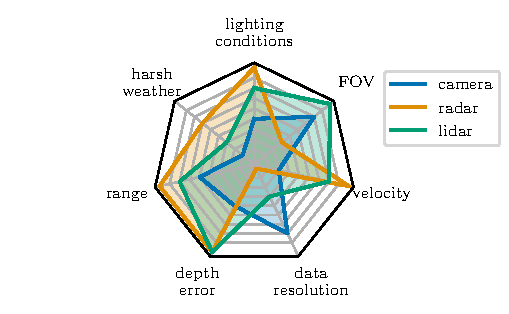
\includegraphics{img/spider_sensorcomp.pdf}
\centering
\caption{Figures MUST be in PDF (everything that can be a vector must be a vector) or PNG format to prevent issues with the arXiv upload.}
\label{fig:compare_sensors}
\end{figure}

% \section{Evaluation}
\label{sec:evaluation}


% \section{Conclusion}
\label{sec:conclusion}

Discussion and Outlook
% \section{Acknowledgment}
\label{sec:acknowledgment}

This work results partly from the KIGLIS project supported by the German Federal Ministry of Education and Research (BMBF), grant number 16KIS1231.

% -------------------------- REFERENCES -------------------------------

{\small
\bibliographystyle{IEEEtran}
\bibliography{literature/AllSourcesMHO.bib}
}

\end{document}
